\section{Langkah-Langkah Percobaan}

\subsection*{Percobaan 1: Konfigurasi Router VPN PPTP PC dengan Router}

Praktikum ini dimulai dengan melakukan reset konfigurasi pada perangkat router untuk memastikan tidak ada konfigurasi sebelumnya yang mengganggu jalannya praktikum. Proses ini krusial untuk memulai konfigurasi dari keadaan bersih.

\begin{figure}[H]
\centering
\begin{minipage}[b]{0.45\textwidth}
\includegraphics[width=\textwidth]{P1/img/Reset Router.png}
\caption{Reset Konfigurasi Router}
\label{fig:reset_router}
\end{minipage}
\end{figure}

Setelah proses reset, langkah selanjutnya adalah melakukan login kembali ke router menggunakan aplikasi Winbox. Hal ini penting untuk memulai semua konfigurasi yang diperlukan.

\begin{figure}[H]
\centering
\begin{minipage}[b]{0.45\textwidth}
\includegraphics[width=\textwidth]{P1/img/Login Router.png}
\caption{Login ke Router}
\label{fig:login_router}
\end{minipage}
\end{figure}

Kemudian, konfigurasi DHCP Client dilakukan pada router untuk mendapatkan koneksi internet. Interface ether3 dipilih sebagai antarmuka yang terhubung ke sumber internet, dengan opsi Use Peer DNS dan Use Peer NTP diaktifkan untuk memastikan resolusi nama domain dan sinkronisasi waktu yang tepat.

\begin{figure}[H]
\centering
\begin{minipage}[b]{0.45\textwidth}
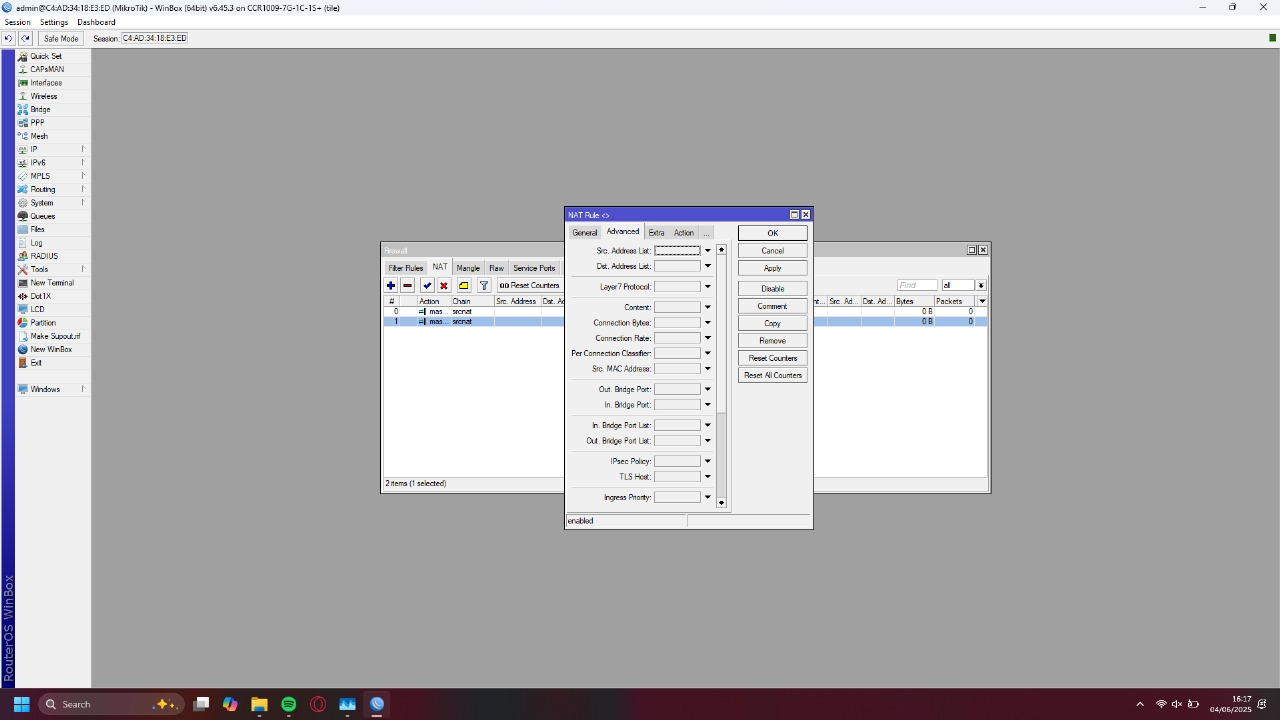
\includegraphics[width=\textwidth]{P1/img/Konfigurasi DHCP Client.jpg}
\caption{Konfigurasi DHCP Client}
\label{fig:dhcp_client}
\end{minipage}
\end{figure}

Langkah berikutnya adalah mengkonfigurasi Firewall NAT (Network Address Translation) untuk memungkinkan perangkat di jaringan lokal dapat mengakses internet. Aturan srcnat dengan Out. Interface ether3 dan Action masquerade diterapkan.

\begin{figure}[H]
\centering
\begin{minipage}[b]{0.45\textwidth}
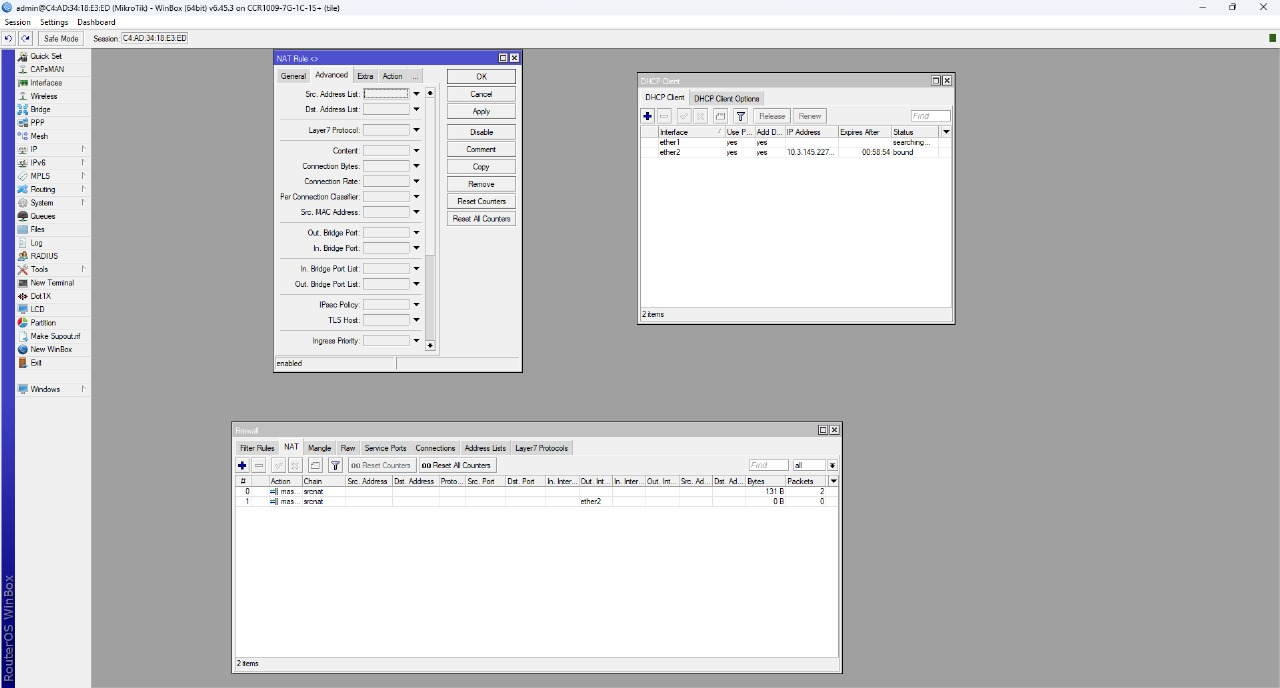
\includegraphics[width=\textwidth]{P1/img/Konfigurasi Firewall NAT.jpg}
\caption{Konfigurasi Firewall NAT}
\label{fig:firewall_nat}
\end{minipage}
\end{figure}

Selanjutnya, alamat IP lokal dikonfigurasi untuk jaringan lokal yang terhubung ke ether1. Alamat IP 192.168.10.2/24 ditetapkan pada antarmuka tersebut.

\begin{figure}[H]
\centering
\begin{minipage}[b]{0.45\textwidth}
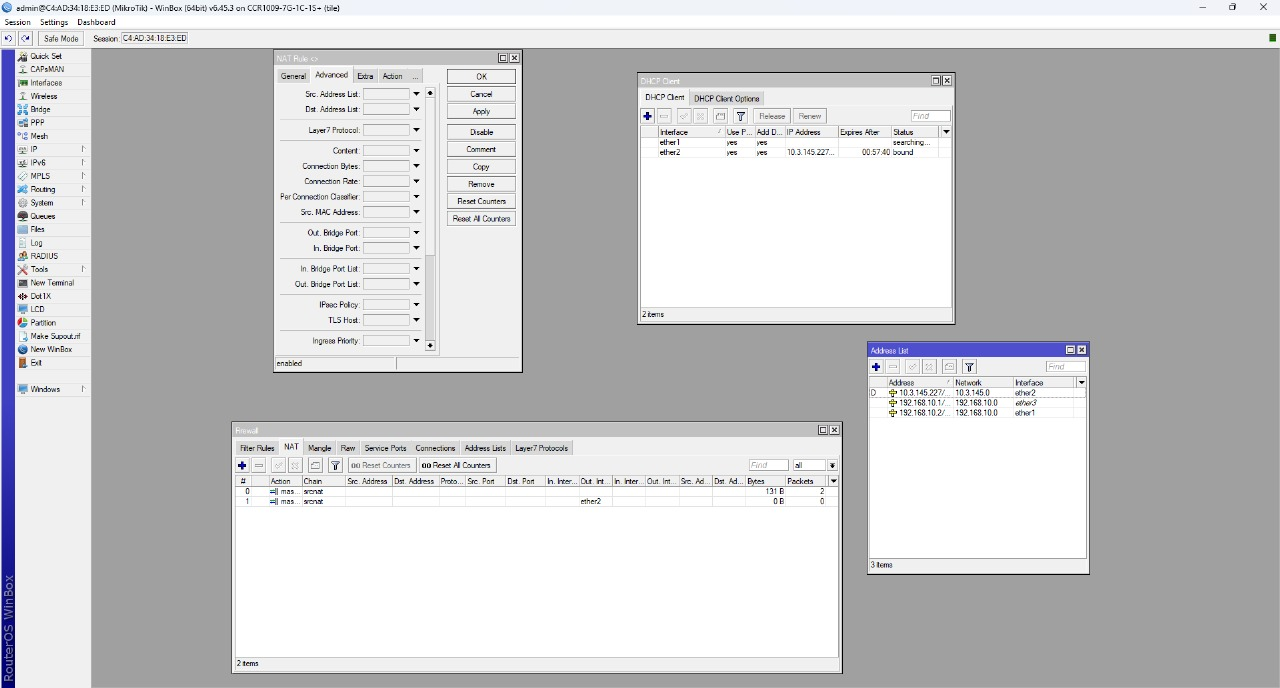
\includegraphics[width=\textwidth]{P1/img/Konfigurasi Alamat IP Lokal.jpg}
\caption{Konfigurasi Alamat IP Lokal}
\label{fig:ip_lokal}
\end{minipage}
\end{figure}

Konfigurasi DHCP Server kemudian dilakukan untuk mendistribusikan alamat IP secara otomatis kepada klien yang terhubung ke ether1. Rentang alamat IP 192.168.10.1−192.168.10.254 ditentukan untuk klien.

\begin{figure}[H]
\centering
\begin{minipage}[b]{0.45\textwidth}
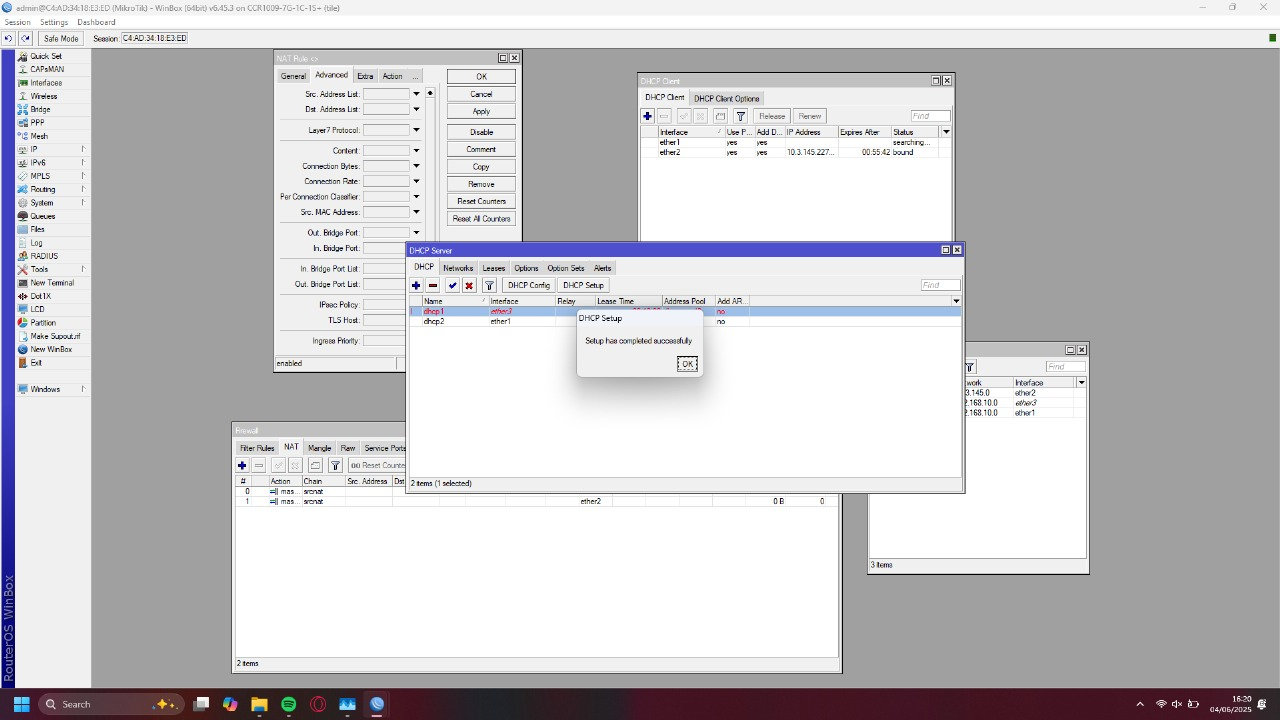
\includegraphics[width=\textwidth]{P1/img/Konfigurasi DHCP Server.jpg}
\caption{Konfigurasi DHCP Server}
\label{fig:dhcp_server}
\end{minipage}
\end{figure}

Untuk mendukung bridging dan routing, mode ARP pada antarmuka ether1 diubah dari enabled menjadi proxy-arp.

\begin{figure}[H]
\centering
\begin{minipage}[b]{0.45\textwidth}
\includegraphics[width=\textwidth]{P1/img/Mengaktifkan Proxy ARP.png}
\caption{Mengaktifkan Proxy ARP}
\label{fig:proxy_arp}
\end{minipage}
\end{figure}

Langkah krusial dalam percobaan VPN PPTP adalah mengaktifkan PPTP Server. Server ini diaktifkan melalui menu PPP pada Winbox.

\begin{figure}[H]
\centering
\begin{minipage}[b]{0.45\textwidth}
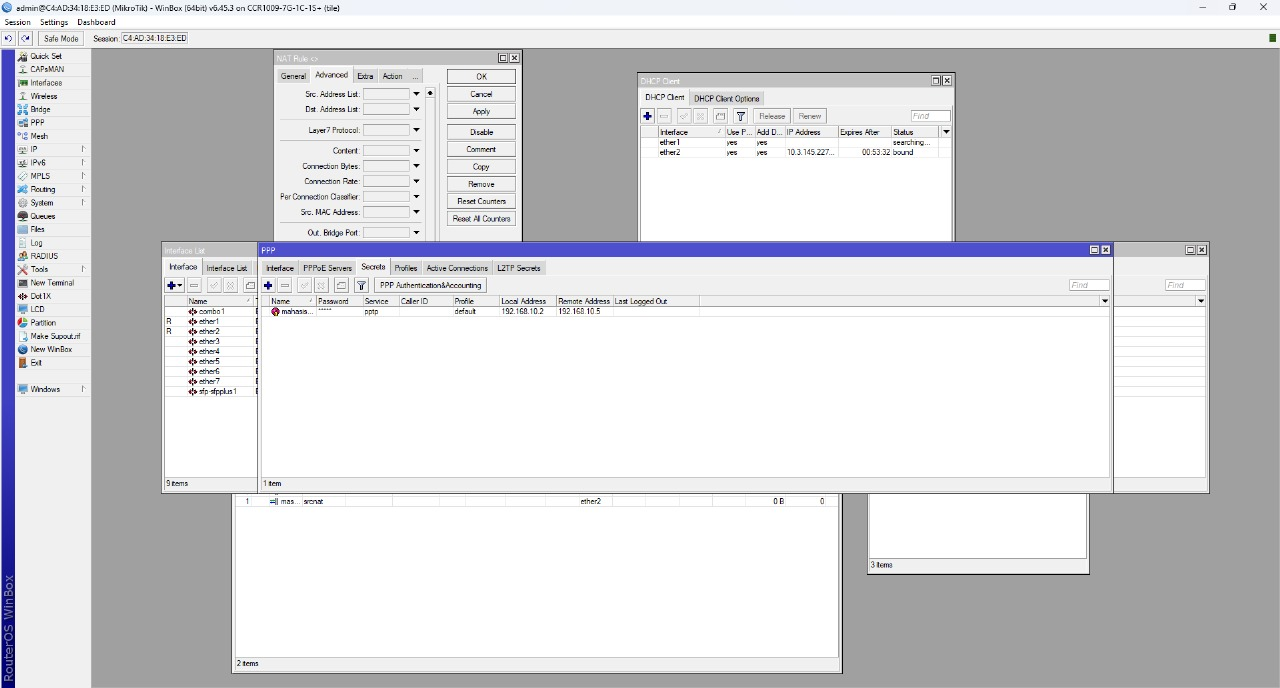
\includegraphics[width=\textwidth]{P1/img/Konfigurasi PPTP Server VPN.jpg}
\caption{Mengaktifkan PPTP Server}
\label{fig:pptp_server}
\end{minipage}
\end{figure}

Kemudian, kredensial pengguna (user dan password) untuk klien VPN dibuat pada tab Secrets. Username "mahasiswa" dengan password "praktikum123" ditetapkan, dengan Local Address 192.168.10.2 dan Remote Address 192.168.10.5.

\begin{figure}[H]
\centering
\begin{minipage}[b]{0.45\textwidth}
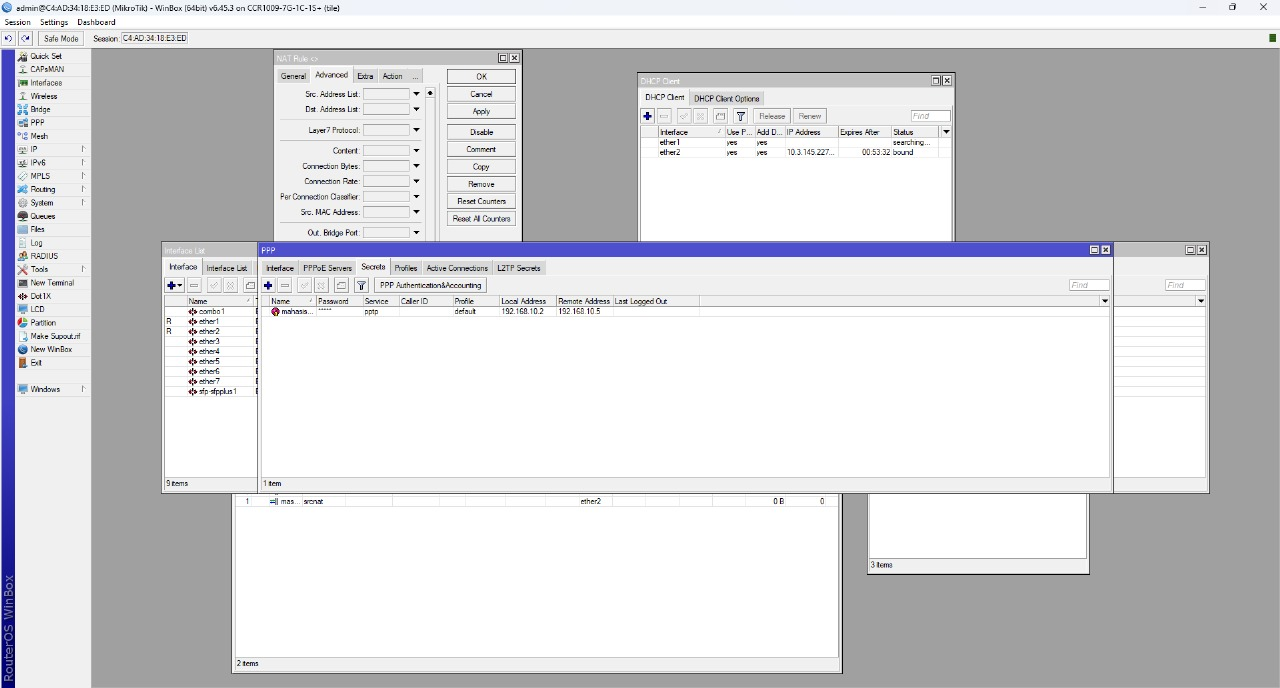
\includegraphics[width=\textwidth]{P1/img/Konfigurasi PPTP Server VPN.jpg}
\caption{Membuat User dan Password (Secrets)}
\label{fig:pptp_secrets}
\end{minipage}
\end{figure}

Terakhir, konfigurasi PPTP Client dilakukan pada laptop (Windows). Koneksi VPN baru ditambahkan dengan detail seperti Server name or address yang merujuk pada IP Address ether3 router, VPN type sebagai Point to Point Tunneling Protocol (PPTP), serta User name dan Password yang telah dibuat sebelumnya.

\begin{figure}[H]
\centering
\begin{minipage}[b]{0.45\textwidth}
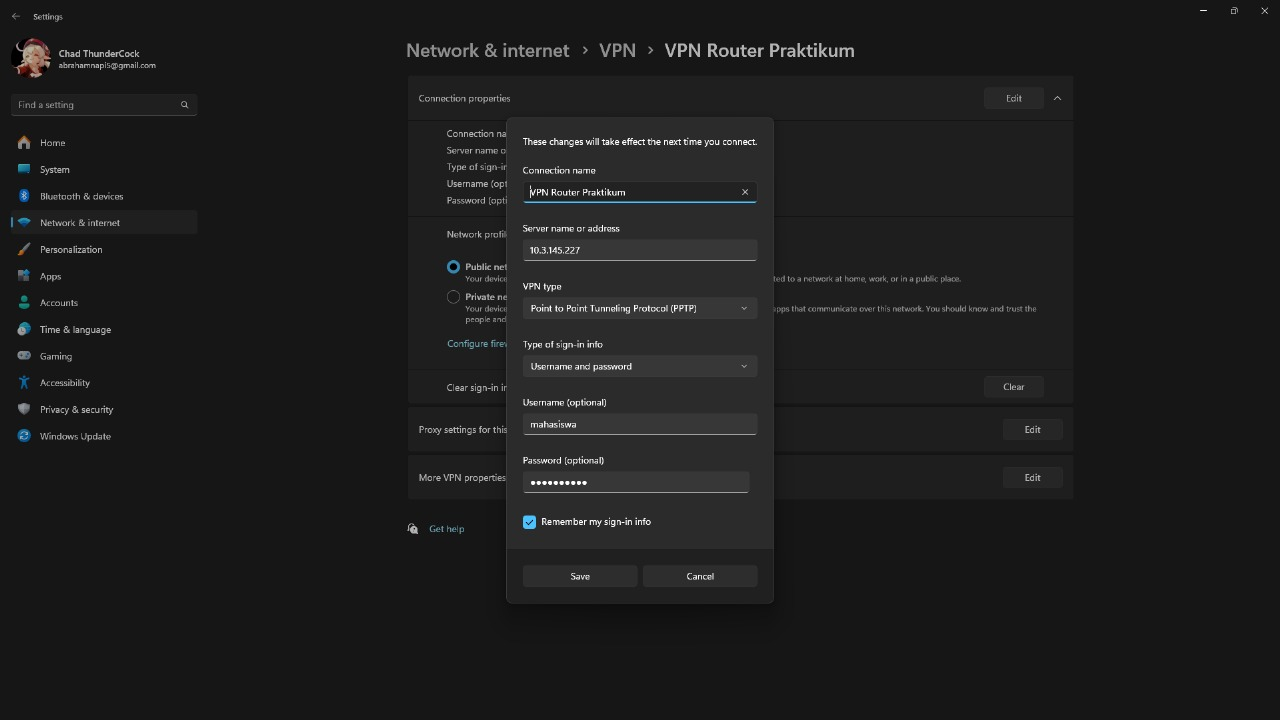
\includegraphics[width=\textwidth]{P1/img/Config VPN PC1.jpg}
\caption{Pengaturan VPN Client (Pengisian Data)}
\label{fig:vpn_client_config}
\end{minipage}
\begin{minipage}[b]{0.45\textwidth}
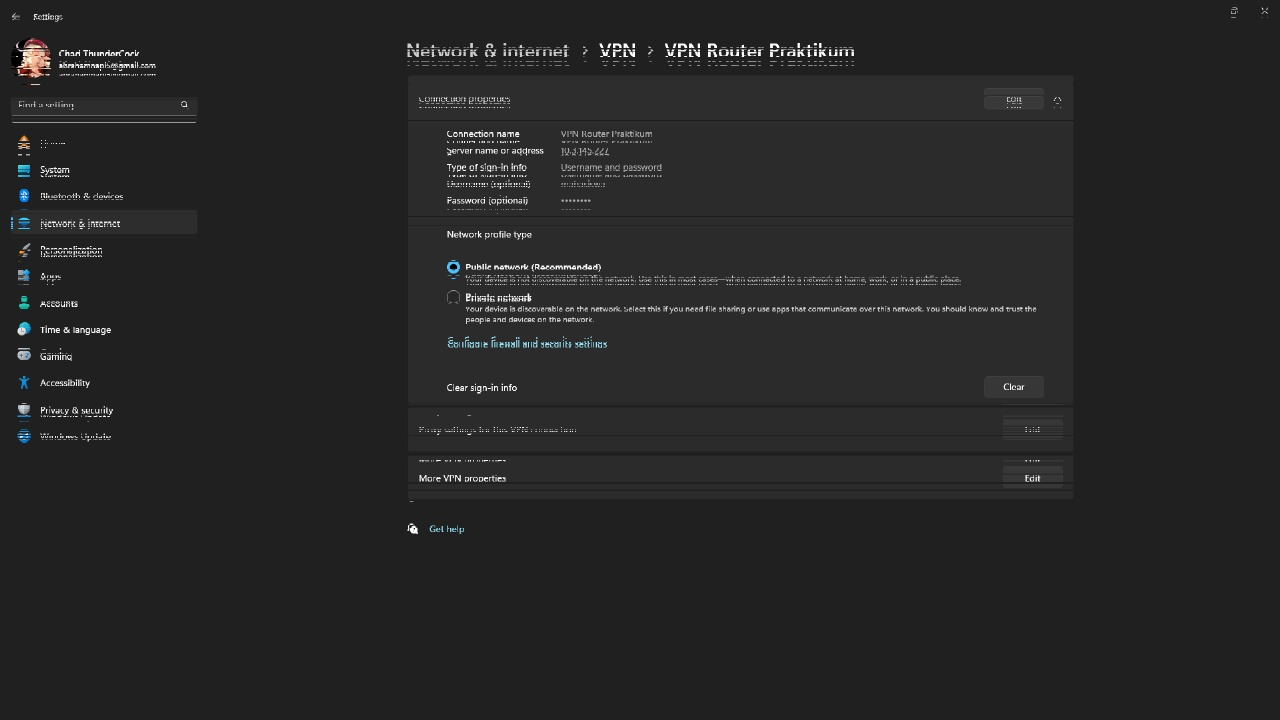
\includegraphics[width=\textwidth]{P1/img/Config VPN 2 PC1.jpg}
\caption{Pengaturan VPN Client (Tampilan Umum)}
\label{fig:vpn_client_overview}
\end{minipage}
\end{figure}

Setelah konfigurasi client VPN di laptop, dilakukan verifikasi koneksi dengan memeriksa ipconfig dan melakukan ping ke alamat IP lokal router. Namun, pada langkah ini, ping selalu mengalami kegagalan.

\begin{figure}[H]
\centering
\begin{minipage}[b]{0.45\textwidth}
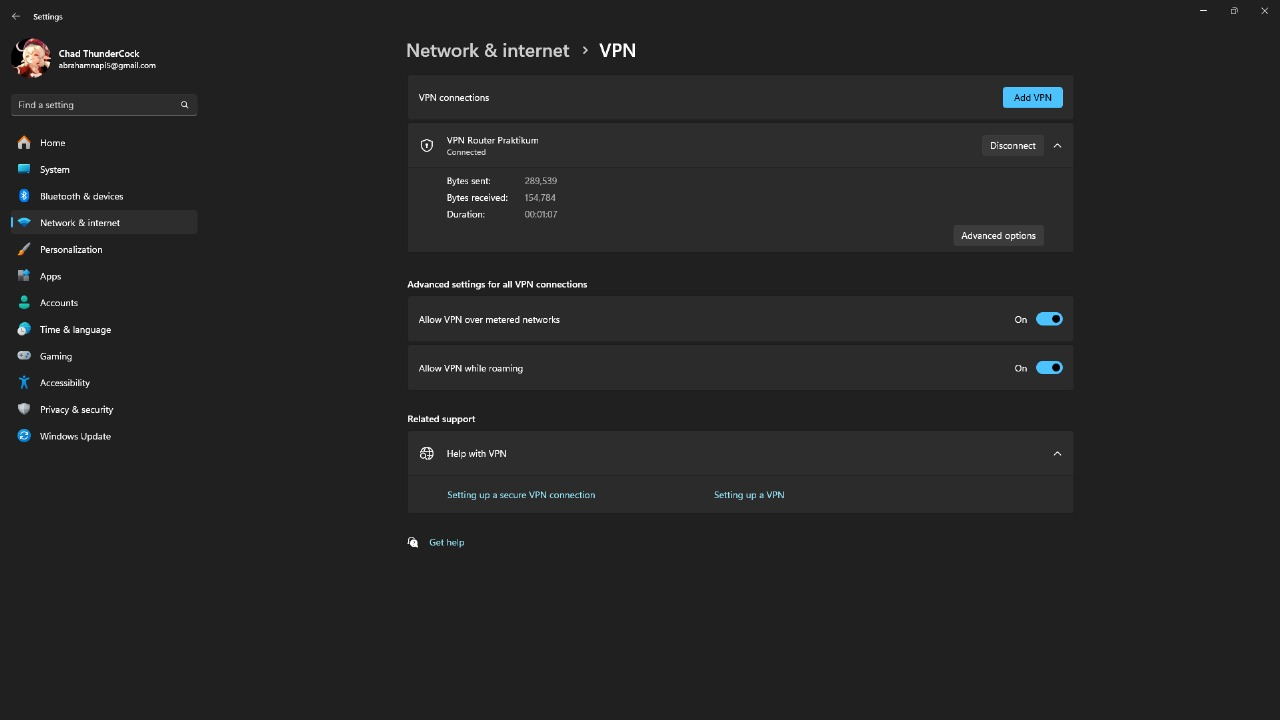
\includegraphics[width=\textwidth]{P1/img/IPconfig PC1.jpg}
\caption{Verifikasi IPconfig PC1}
\label{fig:ipconfig_pc1}
\end{minipage}
\begin{minipage}[b]{0.45\textwidth}
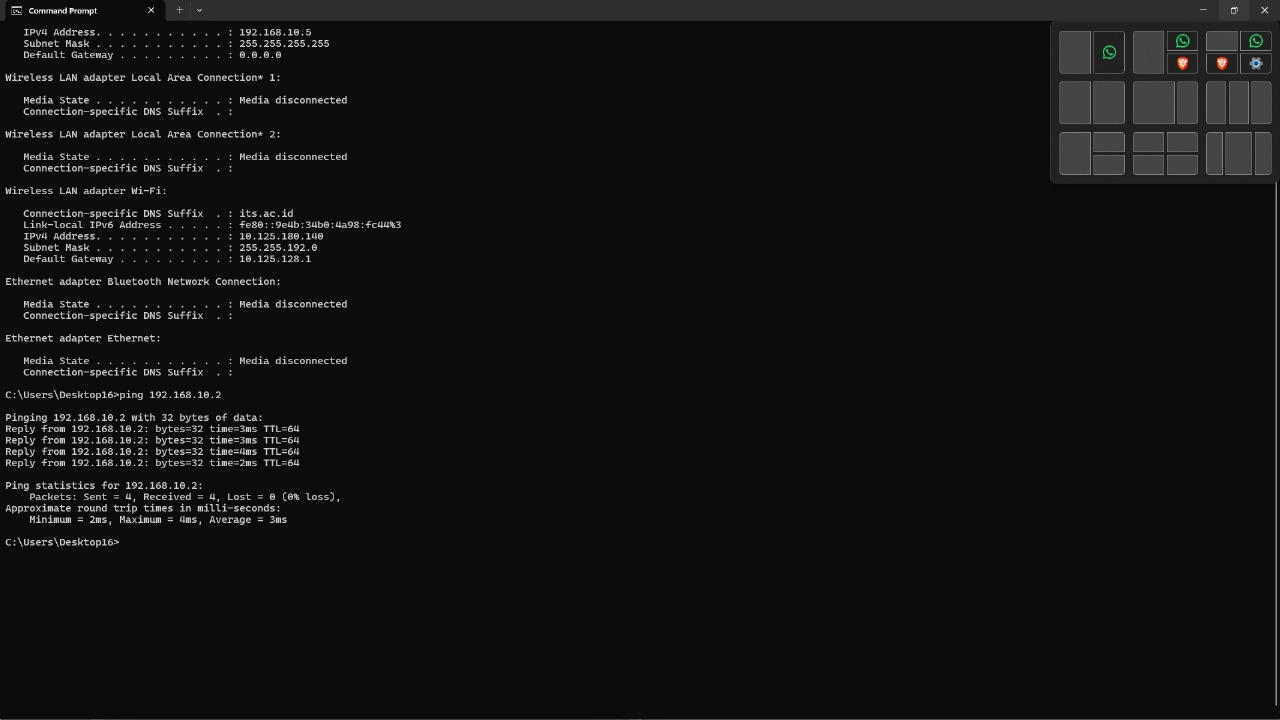
\includegraphics[width=\textwidth]{P1/img/Ping To Router.jpg}
\caption{Ping ke Router (PC 1)}
\label{fig:ping_to_router}
\end{minipage}
\begin{minipage}[b]{0.45\textwidth}
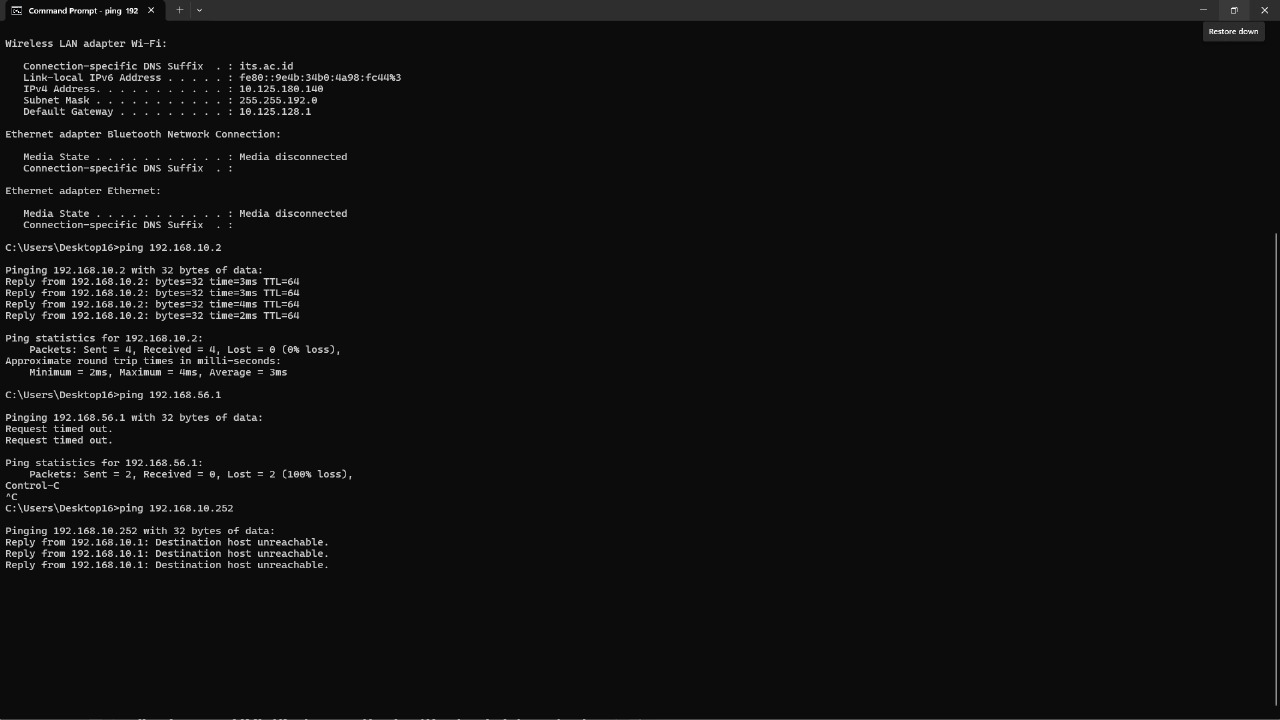
\includegraphics[width=\textwidth]{P1/img/Ping Failed.jpg}
\caption{Ping Gagal (Berbagai Target)}
\label{fig:ping_failed}
\end{minipage}
\begin{minipage}[b]{0.45\textwidth}
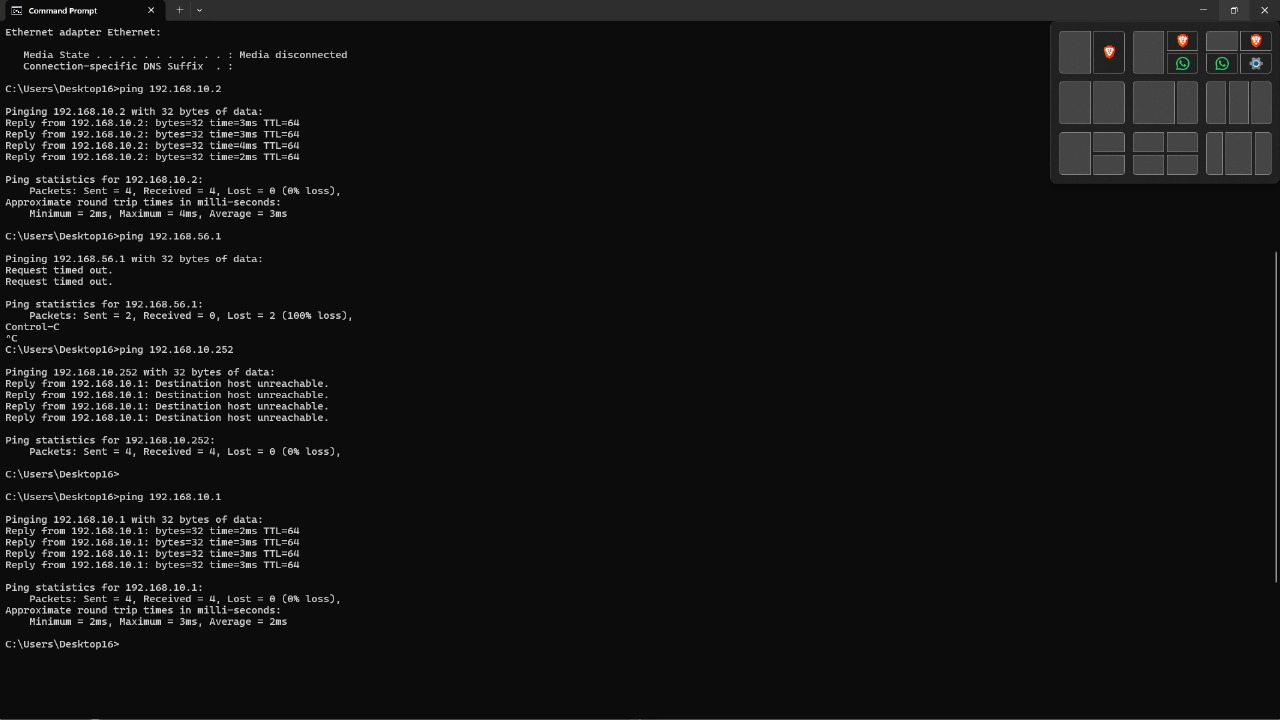
\includegraphics[width=\textwidth]{P1/img/Ping.jpg}
\caption{Ping (Target 192.168.10.1 dan 192.168.10.2)}
\label{fig:ping_success_failure}
\end{minipage}
\end{figure}

\subsection*{Percobaan 2: Konfigurasi QOS PC dengan Router}

Pada percobaan kedua, dilakukan konfigurasi Quality of Service (QoS) menggunakan Simple Queue tanpa perlu mereset konfigurasi router sebelumnya.

Langkah awal adalah membuat aturan Simple Queue untuk membatasi kecepatan upload dan download bagi klien. Aturan Limit-PC-Klien dibuat dengan target jaringan 192.168.10.0/24 dan Max Limit untuk upload dan download masing-masing 1 Mbps.

\begin{figure}[H]
\centering
\begin{minipage}[b]{0.45\textwidth}
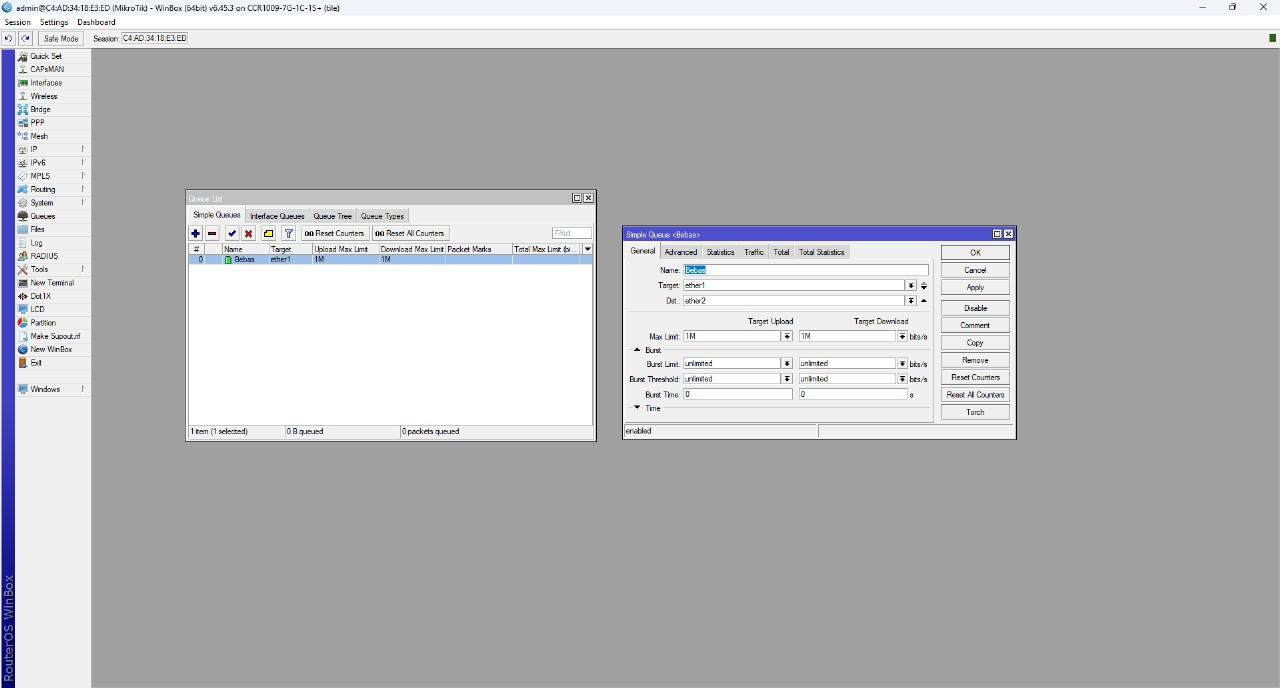
\includegraphics[width=\textwidth]{P1/img/Settingan Queue.jpg}
\caption{Membuat Aturan Simple Queue}
\label{fig:simple_queue}
\end{minipage}
\end{figure}

Kemudian, pemantauan penggunaan traffic dilakukan melalui tab Traffic pada aturan Simple Queue untuk memastikan bahwa pembatasan kecepatan berfungsi secara real-time.

\begin{figure}[H]
\centering
\begin{minipage}[b]{0.45\textwidth}
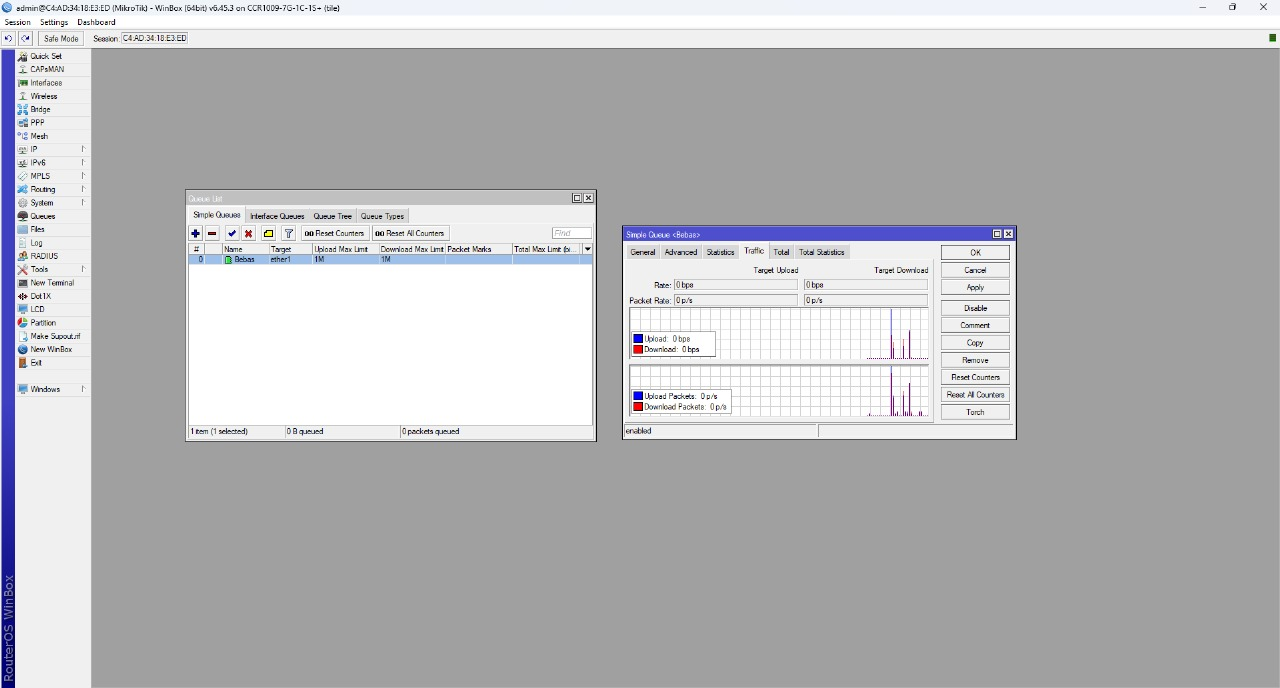
\includegraphics[width=\textwidth]{P1/img/Penggunaan Traffic.jpg}
\caption{Memantau Penggunaan Traffic}
\label{fig:monitor_traffic}
\end{minipage}
\end{figure}

Pengujian efektivitas queue dilakukan dengan membandingkan kecepatan internet sebelum dan sesudah aturan queue diaktifkan. Saat aturan Limit-PC-Klien dinonaktifkan, tes kecepatan internet dijalankan dan hasilnya dicatat.

\begin{figure}[H]
\centering
\begin{minipage}[b]{0.45\textwidth}
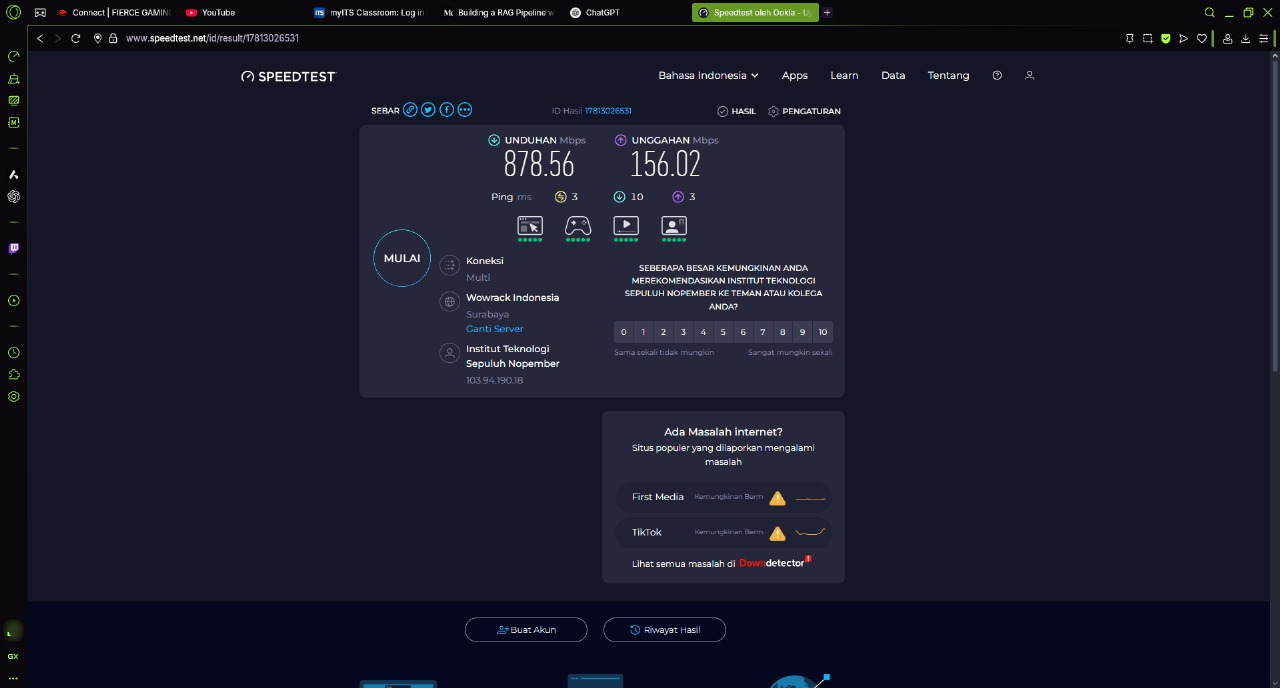
\includegraphics[width=\textwidth]{P1/img/Speedtest saat Queue Nonaktif.jpg}
\caption{Tes Saat Queue Tidak Aktif}
\label{fig:queue_disabled}
\end{minipage}
\end{figure}

Selanjutnya, aturan Limit-PC-Klien diaktifkan kembali, dan tes kecepatan internet dijalankan sekali lagi untuk membandingkan hasilnya.

\begin{figure}[H]
\centering
\begin{minipage}[b]{0.45\textwidth}
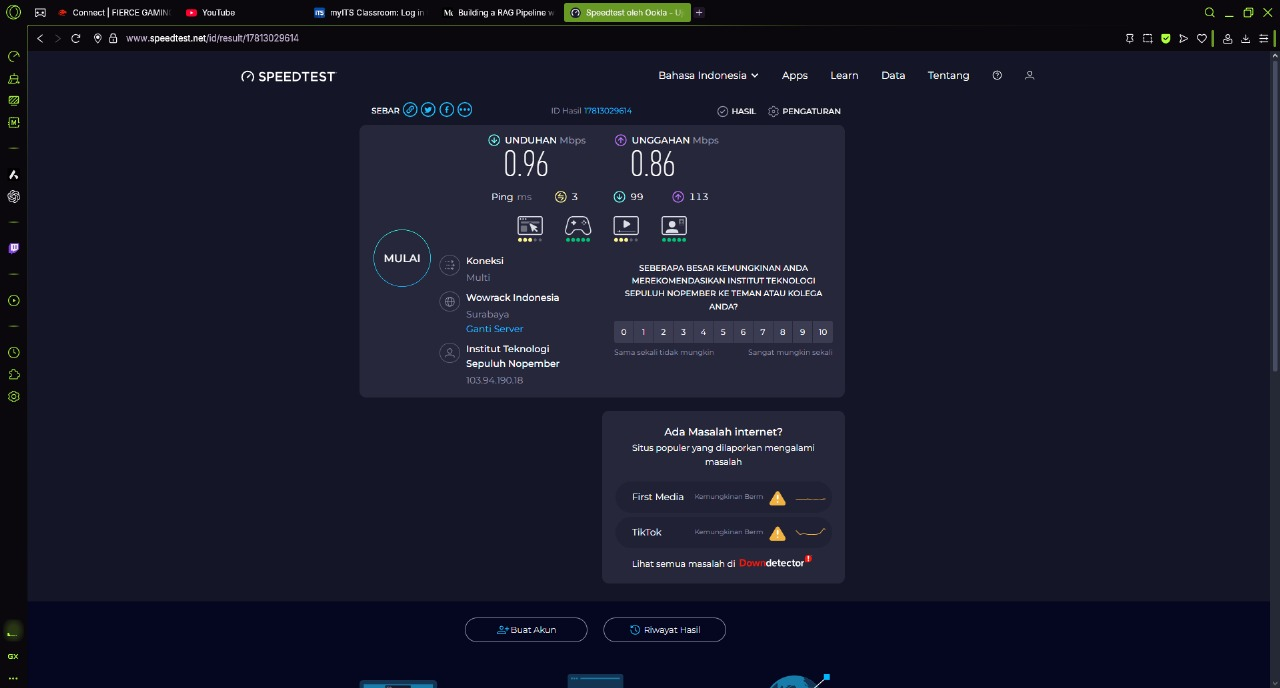
\includegraphics[width=\textwidth]{P1/img/Speedtest saat Queue Aktif.jpg}
\caption{Tes Saat Queue Aktif}
\label{fig:queue_enabled}
\end{minipage}
\end{figure}


\section{Analisis Hasil Percobaan}

\subsection*{Percobaan 1: Konfigurasi Router VPN PPTP PC dengan Router}

Pada percobaan konfigurasi VPN PPTP, seluruh langkah-langkah konfigurasi pada router MikroTik, mulai dari reset konfigurasi, setup DHCP Client untuk koneksi internet, konfigurasi Firewall NAT, penetapan alamat IP lokal, setup DHCP Server untuk distribusi IP ke klien, hingga pengaktifan Proxy ARP dan konfigurasi PPTP Server (termasuk pembuatan user dan password), telah berhasil dilaksanakan sesuai prosedur. Konfigurasi PPTP Client pada sistem operasi Windows juga berhasil dilakukan dengan memasukkan detail koneksi yang sesuai, seperti nama koneksi, alamat server, tipe VPN (PPTP), serta kredensial pengguna.

Namun, kendala signifikan ditemui pada tahap verifikasi dan pengujian, khususnya pada langkah 9. Ketika dilakukan perintah ping dari PC yang terhubung VPN ke alamat IP lokal router (192.168.10.2), ping selalu mengalami kegagalan (terlihat dari Request timed out atau Destination host unreachable pada berbagai percobaan ping seperti ke 192.168.56.1 dan 192.168.10.252 serta ke 192.168.10.1 pada salah satu screenshot meskipun ping ke 192.168.10.2 ada yang berhasil pada screenshot lain). Hal ini mengindikasikan bahwa meskipun konfigurasi VPN pada kedua sisi (server dan klien) telah diselesaikan secara sintaksis, terdapat masalah pada konektivitas atau rute jaringan melalui tunnel VPN. Potensi penyebab kegagalan ini meliputi masalah pada konfigurasi routing di router setelah VPN terbentuk, isu pada firewall yang mungkin memblokir lalu lintas PPTP atau ICMP melalui tunnel, atau kemungkinan adanya inkonsistensi pada alamat IP yang ditetapkan untuk Remote Address di PPTP Secrets (192.168.10.5) dan alamat IP yang diharapkan oleh klien setelah koneksi VPN terbentuk. Kegagalan ping pada sebagian besar percobaan menunjukkan bahwa komunikasi dasar antara klien VPN dan jaringan lokal di balik router VPN tidak dapat terjalin secara konsisten, sehingga tujuan utama dari VPN (yaitu ekstensi jaringan) tidak tercapai sepenuhnya.

\subsection*{Percobaan 2: Konfigurasi QOS PC dengan Router}

Pada percobaan konfigurasi Quality of Service (QoS) menggunakan Simple Queue, seluruh langkah-langkah berhasil dieksekusi dengan baik. Pembuatan aturan Simple Queue dengan nama Limit-PC-Klien pada target jaringan 192.168.10.0/24 dan pengaturan Max Limit sebesar 1 Mbps untuk upload dan download telah berhasil diimplementasikan, seperti yang terlihat pada screenshot Settingan Queue.jpg. Pemantauan penggunaan traffic pada tab Traffic juga menunjukkan bahwa aturan queue berfungsi secara real-time, mengindikasikan adanya manajemen bandwidth, yang terlihat pada screenshot Penggunaan Traffic.jpg.

Hasil pengujian efektivitas queue menunjukkan keberhasilan yang jelas. Ketika aturan Limit-PC-Klien dinonaktifkan, kecepatan internet yang terukur pada PC klien menunjukkan unduhan 878.56 Mbps dan unggahan 156.02 Mbps (Speedtest saat Queue Nonaktif.jpg), cenderung mendekati kecepatan maksimum yang disediakan oleh ISP atau jaringan lokal. Sebaliknya, saat aturan Limit-PC-Klien diaktifkan kembali, kecepatan download dan upload pada PC klien secara signifikan terbatas, dengan unduhan 0.96 Mbps dan unggahan 0.86 Mbps (Speedtest saat Queue Aktif.jpg), mendekati nilai 1 Mbps yang telah dikonfigurasi. Hal ini membuktikan bahwa Simple Queue telah bekerja sesuai dengan tujuan, yaitu membatasi bandwidth untuk traffic yang ditargetkan. Keberhasilan ini menunjukkan pemahaman yang baik dalam penerapan kebijakan Quality of Service untuk mengelola penggunaan bandwidth dalam suatu jaringan.
\section*{Hasil Tugas Modul}

\subsection*{1. Topologi Jaringan}
Topologi jaringan yang dibangun dalam simulasi ini adalah sebagai berikut: PC0 terhubung ke Router0 melalui Switch0, dan PC1 terhubung ke Router1 melalui Switch1. Kedua router, Router0 dan Router1, dihubungkan melalui sebuah Switch yang berfungsi sebagai simulasi jaringan internet. Koneksi antara Router0 dan Router1 membentuk Virtual Private Network (VPN) menggunakan GRE Tunnel.

\begin{figure}[h!]
    \centering
    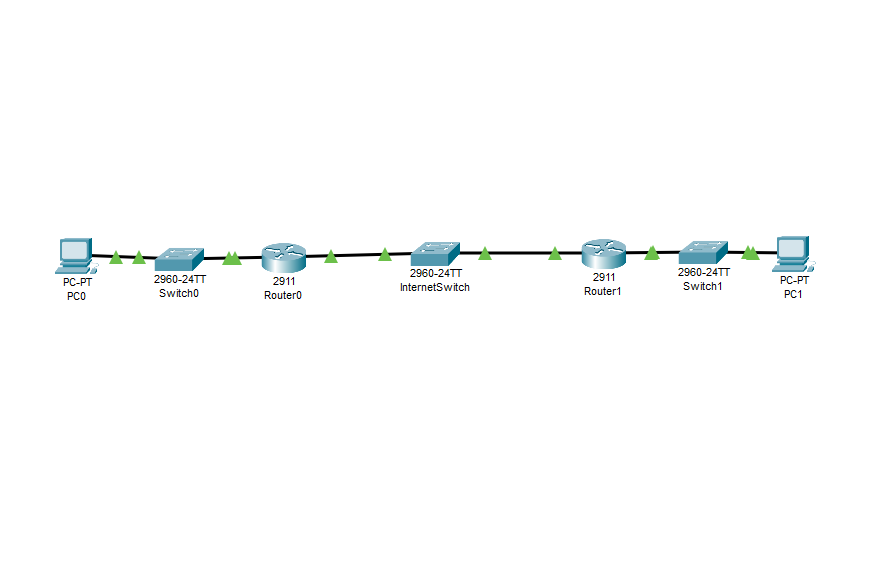
\includegraphics[width=0.9\textwidth]{P1/img/Topologi (3).png} 
    \caption{Topologi Jaringan Simulasi}
    \label{fig:topologi}
\end{figure}

\subsection*{2. Pengaturan IP Address}
Berikut adalah skema IP address yang digunakan dalam simulasi:
\begin{itemize}
    \item \textbf{Jaringan Lokal 1 (PC0 - Switch0 - Router0):} 192.168.1.0/24
    \begin{itemize}
        \item PC0: \texttt{192.168.1.2}
        \item Router0 (GigabitEthernet0/0 - LAN): \texttt{192.168.1.1}
    \end{itemize}
    \item \textbf{Jaringan Internet (Router0 - Internet-Switch - Router1):} 203.0.113.0/24
    \begin{itemize}
        \item Router0 (GigabitEthernet0/1 - WAN): \texttt{203.0.113.1}
        \item Router1 (GigabitEthernet0/1 - WAN): \texttt{203.0.113.2}
    \end{itemize}
    \item \textbf{Jaringan Lokal 2 (PC1 - Switch1 - Router1):} 192.168.2.0/24
    \begin{itemize}
        \item PC1: \texttt{192.168.2.2}
        \item Router1 (GigabitEthernet0/0 - LAN): \texttt{192.168.2.1}
    \end{itemize}
    \item \textbf{Jaringan GRE Tunnel:} 10.0.0.0/30
    \begin{itemize}
        \item Interface Tunnel di Router0: \texttt{10.0.0.1}
        \item Interface Tunnel di Router1: \texttt{10.0.0.2}
    \end{itemize}
\end{itemize}

Konfigurasi IP pada Router0 dan Router1 dapat dilihat pada Lampiran \ref{lampiran:ip_router0} dan \ref{lampiran:ip_router1}.

\subsection*{3. Konfigurasi GRE Tunnel}
Awalnya, tugas ini bertujuan untuk mengimplementasikan PPTP (Point-to-Point Tunneling Protocol). Namun, dalam simulasi menggunakan Cisco Packet Tracer versi yang digunakan (dan model router 2911), terdapat kendala fungsionalitas di mana perintah PPTP seperti \texttt{tunnel mode pptp} tidak didukung dan menghasilkan pesan error.

\begin{figure}[h!]
    \centering
    \begin{minipage}[t]{0.48\textwidth}
        \centering
        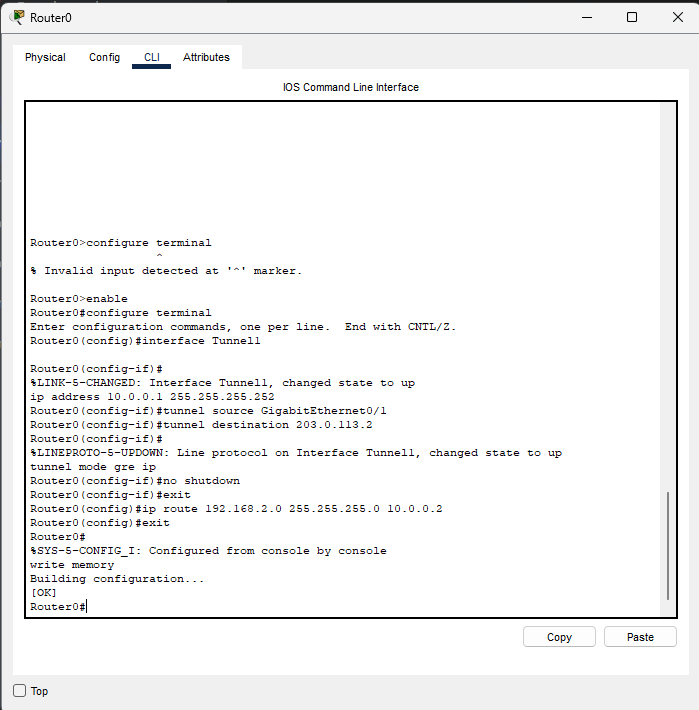
\includegraphics[width=\textwidth]{P1/img/GRE Tunnel Router0.png} 
        \caption{Konfigurasi GRE Tunnel Router0}
        \label{fig:gre_router0}
    \end{minipage}
    \hfill
    \begin{minipage}[t]{0.48\textwidth}
        \centering
        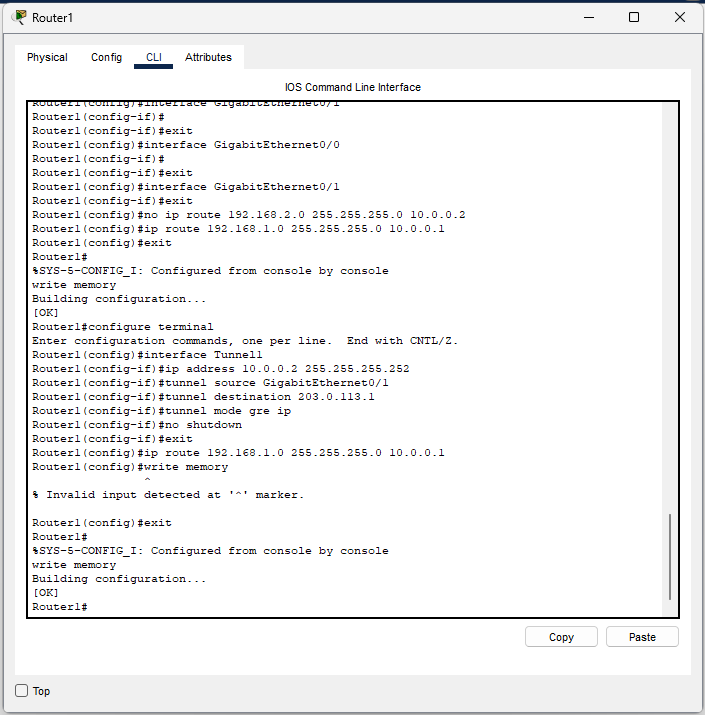
\includegraphics[width=\textwidth]{P1/img/GRE Tunnel Router1.png} 
        \caption{Konfigurasi GRE Tunnel Router1}
        \label{fig:gre_router1}
    \end{minipage}
    \caption{Konfigurasi GRE Tunnel pada Router0 dan Router1}
\end{figure}

Sebagai alternatif, \textbf{GRE (Generic Routing Encapsulation) Tunnel} dipilih untuk menciptakan terowongan VPN antar Router0 dan Router1. GRE adalah protokol tunneling yang membungkus paket data di dalam paket IP lain, memungkinkan data dari satu protokol jaringan untuk melewati jaringan lain. Meskipun GRE tidak menyediakan enkripsi secara bawaan seperti PPTP, ia berhasil membangun konektivitas virtual antara dua jaringan lokal melalui simulasi internet.

Konfigurasi GRE Tunnel pada Router0 dan Router1 adalah sebagai berikut:
\begin{itemize}
    \item \textbf{Router0 (Server/Source Tunnel):}
    \begin{verbatim}
        interface Tunnel1
        ip address 10.0.0.1 255.255.255.252
        tunnel source GigabitEthernet0/1
        tunnel destination 203.0.113.2
        tunnel mode gre ip
        no shutdown
        ip route 192.168.2.0 255.255.255.0 10.0.0.2
    \end{verbatim}
    \item \textbf{Router1 (Client/Destination Tunnel):}
    \begin{verbatim}
        interface Tunnel1
        ip address 10.0.0.2 255.255.255.252
        tunnel source GigabitEthernet0/1
        tunnel destination 203.0.113.1
        tunnel mode gre ip
        no shutdown
        ip route 192.168.1.0 255.255.255.0 10.0.0.1
    \end{verbatim}
\end{itemize}

\subsection*{4. Hasil Pengujian Konektivitas (Ping Test)}
Setelah konfigurasi GRE Tunnel diterapkan dan disimpan pada kedua router, pengujian konektivitas dilakukan dari PC0 ke PC1, dan sebaliknya. Pengujian ini dilakukan untuk memastikan bahwa kedua jaringan lokal dapat saling berkomunikasi melalui tunnel VPN.

\begin{figure}[h!]
    \centering
    \begin{minipage}[t]{0.48\textwidth}
        \centering
        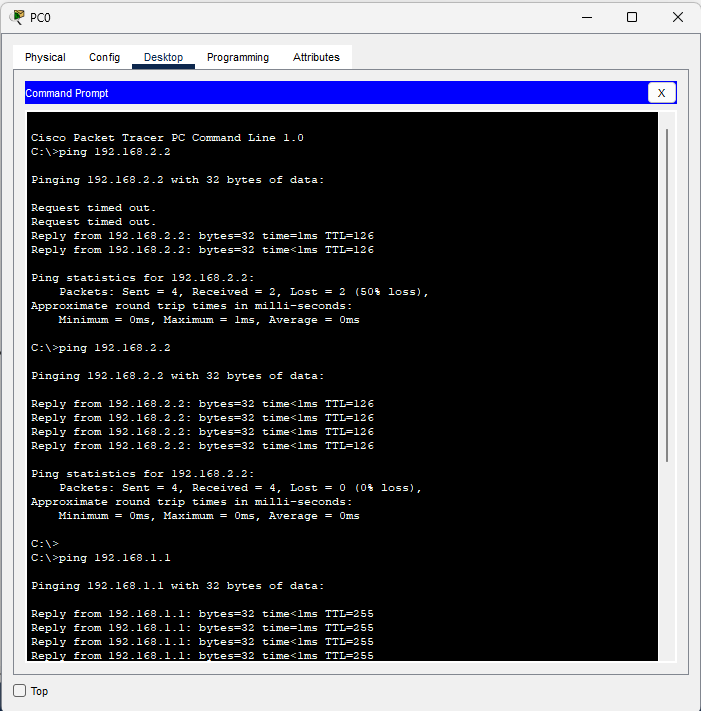
\includegraphics[width=\textwidth]{P1/img/Test Ping GRE Tunnel PC0 ke PC1.png} 
        \caption{Ping dari PC0 ke PC1}
        \label{fig:ping_pc0_pc1}
    \end{minipage}
    \hfill
    \begin{minipage}[t]{0.48\textwidth}
        \centering
        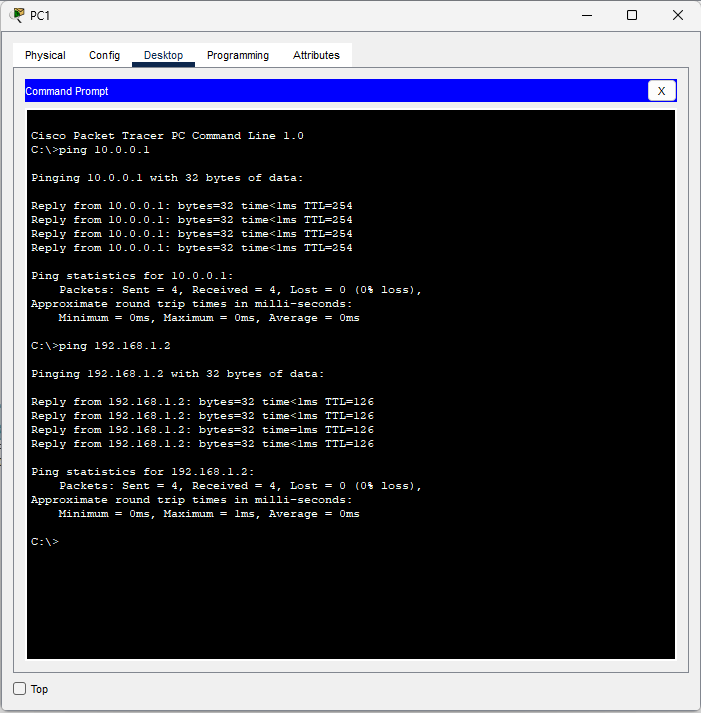
\includegraphics[width=\textwidth]{P1/img/Test Ping GRE Tunnel PC1 ke PC0 .png} 
        \caption{Ping dari PC1 ke PC0}
        \label{fig:ping_pc1_pc0}
    \end{minipage}
    \caption{Hasil Pengujian Konektivitas PC0 dan PC1}
\end{figure}

Seperti yang terlihat pada Gambar \ref{fig:ping_pc0_pc1} dan \ref{fig:ping_pc1_pc0}, setelah beberapa percobaan awal (yang normalnya mungkin mengalami \texttt{Request timed out} karena proses ARP dan konvergensi), ping berhasil 100\% dari PC0 ke PC1, dan juga dari PC1 ke PC0. Ini menunjukkan bahwa GRE Tunnel telah berhasil dibangun dan menyediakan jalur komunikasi antara kedua jaringan yang terpisah.

\subsection*{5. Penjelasan Singkat tentang Fungsi PPTP dan Kendala}
\textbf{PPTP (Point-to-Point Tunneling Protocol)} adalah protokol jaringan yang digunakan untuk mengimplementasikan Virtual Private Network (VPN). PPTP beroperasi pada lapisan data-link (Layer 2) dan menggunakan TCP port 1723 untuk menginisialisasi tunnel serta GRE (Generic Routing Encapsulation) untuk membawa paket data yang dienkapsulasi. Fungsi utamanya adalah membuat "terowongan" virtual melalui jaringan publik (seperti internet) untuk mengirim data, mengenkapsulasi data asli, dan menyediakan keamanan melalui otentikasi dan enkripsi (meskipun PPTP modern dianggap kurang aman dibandingkan IPSec atau OpenVPN).

Dalam tugas ini, kendala utama yang dihadapi adalah \textbf{keterbatasan Cisco Packet Tracer} dalam mendukung implementasi PPTP secara penuh pada model router yang digunakan (2911). Perintah konfigurasi PPTP spesifik seperti \texttt{tunnel mode pptp} tidak dikenali oleh perangkat lunak, menyebabkan error. Selain itu, komponen \texttt{Cloud-PT-Empty} yang seharusnya mensimulasikan Internet, juga menunjukkan perilaku yang tidak diharapkan, di mana port Ethernet yang ditambahkan masih terikat pada opsi Cable/DSL, bukan koneksi Ethernet murni yang diperlukan.

Oleh karena kendala tersebut, diputuskan untuk:
\begin{itemize}
    \item Mengganti komponen \texttt{Cloud} dengan sebuah \textbf{Switch 2960} yang dinamai \texttt{InternetSwitch}. Switch ini berfungsi sebagai media perantara Layer 2 yang sederhana dan stabil untuk menghubungkan dua router melalui jaringan yang merepresentasikan "internet".
    \item Mengganti protokol VPN dari PPTP menjadi \textbf{GRE Tunnel}. GRE Tunnel terbukti berfungsi dengan baik di Cisco Packet Tracer dan berhasil membangun konektivitas virtual antar kedua jaringan, memenuhi tujuan utama tugas untuk mensimulasikan VPN.
\end{itemize}
Meskipun terjadi perubahan protokol, simulasi ini tetap berhasil menunjukkan konsep dasar pembuatan tunnel VPN antar dua jaringan yang terpisah.

\newpage
\appendix
\section*{Lampiran Screenshot Konfigurasi}

\begin{figure}[h!]
    \centering
    \begin{minipage}[t]{0.48\textwidth}
        \centering
        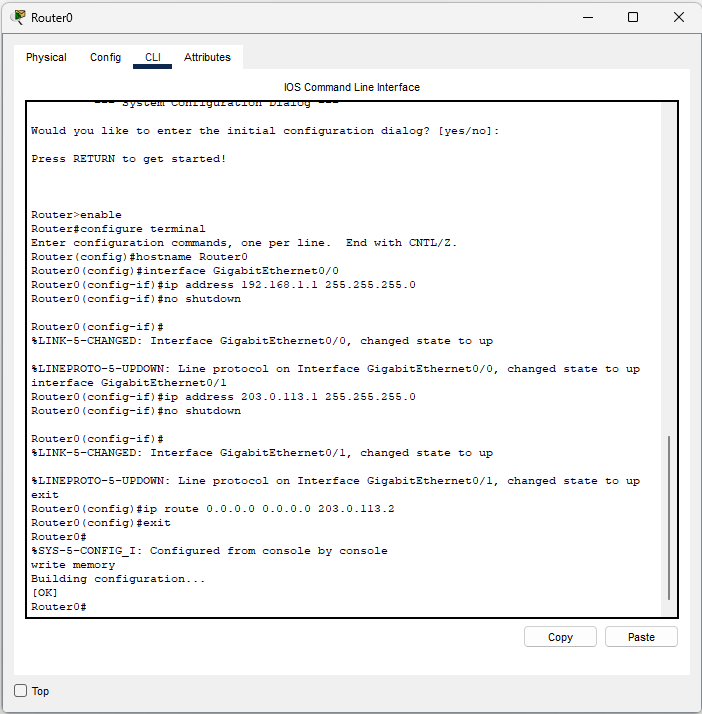
\includegraphics[width=\textwidth]{P1/img/IP Router0.png} 
        \caption{Konfigurasi IP Router0}
        \label{lampiran:ip_router0}
    \end{minipage}
    \hfill
    \begin{minipage}[t]{0.48\textwidth}
        \centering
        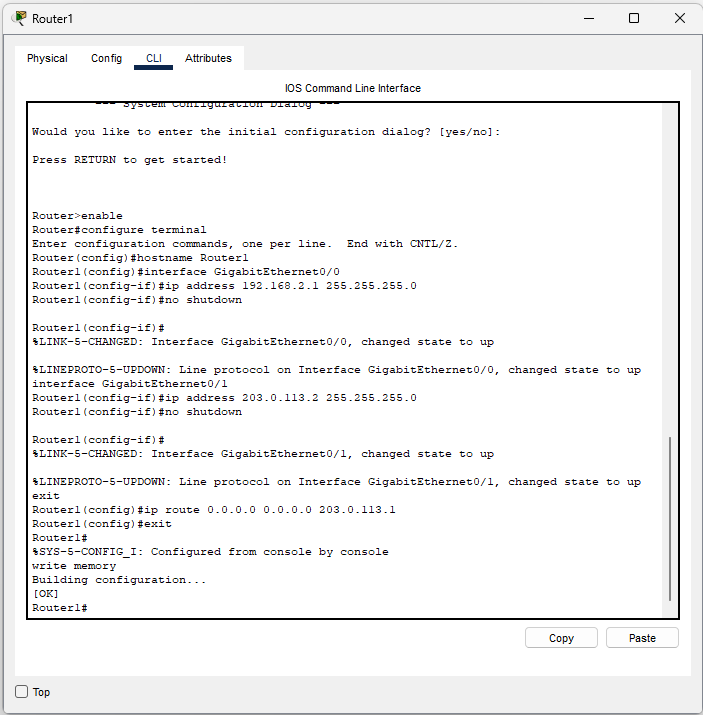
\includegraphics[width=\textwidth]{P1/img/IP Router1.png} 
        \caption{Konfigurasi IP Router1}
        \label{lampiran:ip_router1}
    \end{minipage}
    \caption{Konfigurasi IP Address pada Router}
\end{figure}

\section*{Kesimpulan}

Praktikum ini berhasil mengimplementasikan berbagai aspek penting dalam jaringan komputer, meliputi konfigurasi VPN PPTP dan Quality of Service (QoS). Pada percobaan VPN PPTP, meskipun semua tahapan konfigurasi pada router MikroTik dan klien Windows telah dieksekusi secara sintaksis, konektivitas akhir yang diverifikasi dengan ping mengalami kegagalan pada beberapa percobaan. Hal ini menunjukkan adanya potensi isu pada lapisan jaringan atau firewall yang menghambat komunikasi melalui tunnel VPN, meskipun parameter konfigurasi awal telah disiapkan. Kegagalan ping mengindikasikan bahwa meskipun tunnel secara teknis mungkin telah terbentuk, aliran data yang sebenarnya belum dapat melewati tunnel dengan sukses secara konsisten.

Di sisi lain, percobaan konfigurasi Quality of Service (QoS) menggunakan Simple Queue menunjukkan keberhasilan yang signifikan. Pembatasan bandwidth untuk upload dan download telah berhasil diterapkan dan diverifikasi melalui pengujian kecepatan internet. Hasil pengujian secara konsisten menunjukkan bahwa kecepatan dibatasi sesuai dengan parameter yang telah dikonfigurasi, membuktikan efektivitas Simple Queue dalam manajemen bandwidth. Hal ini menegaskan pemahaman dan kemampuan dalam mengimplementasikan kebijakan QoS untuk mengatur penggunaan sumber daya jaringan secara efisien.

Selain itu, analisis terhadap lampiran konfigurasi GRE Tunnel menunjukkan pemahaman dalam membangun konektivitas point-to-point yang aman antara dua router. Konfigurasi ini, yang meliputi penetapan alamat IP, penentuan sumber dan tujuan tunnel, serta penambahan rute statis, adalah fundamental dalam membangun jaringan virtual pribadi yang terenkapsulasi. Meskipun tidak ada hasil pengujian yang disertakan untuk GRE Tunnel, detail konfigurasi menunjukkan implementasi yang logis dan sesuai dengan prinsip-prinsip tunneling GRE.

Secara keseluruhan, praktikum ini memberikan pengalaman berharga dalam konfigurasi jaringan, meskipun terdapat tantangan pada implementasi VPN PPTP yang memerlukan analisis lebih lanjut untuk identifikasi akar masalahnya. Keberhasilan dalam konfigurasi QoS dan pemahaman terhadap GRE Tunnel menunjukkan kompetensi yang kuat dalam administrasi jaringan.